\section{Inheritance procedure}

\bfr{Problems with a natural tree structure}
  \bb{Genetic association studies}
      -$\circ$ Whole genome
    \\---$\circ$ chromosomes
    \\-----$\circ$ genes
  \eb
  \pause
  \bb{Self Report psychological/sociological questionnaires}
      -$\circ$ investigated concepts
    \\---$\circ$ different aspects
    \\-----$\circ$ single items (questions)
  \eb
  \pause
  \bb{Alternative}
    Make a tree structure from the data by hierarchical clustering
  \eb
\end{frame}




% ==========================
\begin{frame}
\frametitle{Example of Tree-Structured Hypotheses: Genes}

%\begin{figure}
\begin{center}
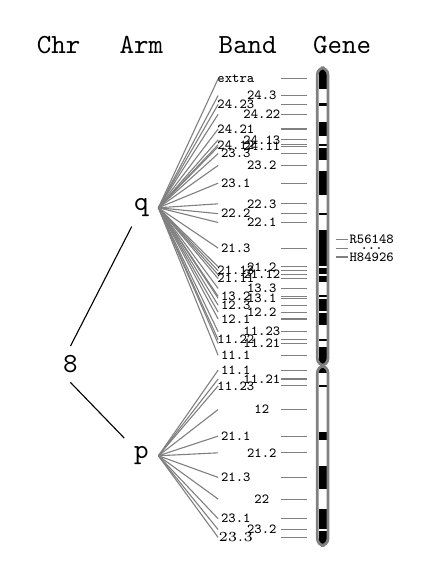
\begin{tikzpicture}
\begin{scope}[scale=.15,yshift=-6cm, font=\ttfamily]

\path  (-4,42.25) node {Chr};			
\path  (3,42.25) node {Arm};			
\path  (12,42.25) node {Band};			
\path  (20,42.25) node {Gene};			
\path  (-3,15.25) node (ch8) { 8};	
\path  (3,7.5) node (p) {p}; \draw  (ch8.south) -- (p);
\path  (3,28.5) node (q) { q};\draw  (ch8.north) -- (q);

\fill		(18,0) rectangle +(.7,1.17);	\path  (11,0.58) node (n1) {\tiny $23.3$} ;
\draw[color=gray]  (14.8,0.583333333333333) -- (17,0.583333333333333);
\draw[color=gray]  (p.east) -- (9.5,0.583333333333333);
\fill	[color=white]	(18,1.17) rectangle +(.7,0.17);	\path  (13.2,1.25) node (n2) {\tiny 23.2} ;
\draw[color=gray]  (14.8,1.25) -- (17,1.25); \draw[color=gray]  (p.east) -- (9.5,1.25);
\fill		(18,1.33) rectangle +(.7,1.67);	\path  (11,2.17) node (n3) {\tiny 23.1} ;
\draw[color=gray]  (14.8,2.16666666666667) -- (17,2.16666666666667); 
\draw[color=gray]  (p.east) -- (9.5,2.16666666666667);
\fill	[color=white]	(18,3) rectangle +(.7,1.67);	\path  (13.2,3.83) node (n4) {\tiny 22} ;
\draw[color=gray]  (14.8,3.83333333333333) -- (17,3.83333333333333); 
\draw[color=gray]  (p.east) -- (9.5,3.83333333333333);
\fill		(18,4.67) rectangle +(.7,2);	\path  (11,5.67) node (n5) {\tiny 21.3} ;
\draw[color=gray]  (14.8,5.66666666666667) -- (17,5.66666666666667);
 \draw[color=gray]  (p.east) -- (9.5,5.66666666666667);
\fill	[color=white]	(18,6.67) rectangle +(.7,2.17);	\path  (13.2,7.75) node (n6) {\tiny 21.2} ;
\draw[color=gray]  (14.8,7.75) -- (17,7.75); \draw[color=gray]  (p.east) -- (9.5,7.75);
\fill		(18,8.83) rectangle +(.7,0.67);	\path  (11,9.17) node (n7) {\tiny 21.1} ;
\draw[color=gray]  (14.8,9.16666666666667) -- (17,9.16666666666667); 
\draw[color=gray]  (p.east) -- (9.5,9.16666666666667);
\fill	[color=white]	(18,9.5) rectangle +(.7,3.83);	\path  (13.2,11.42) node (n8) {\tiny 12} ;
\draw[color=gray]  (14.8,11.4166666666667) -- (17,11.4166666666667);
 \draw[color=gray]  (p.east) -- (9.5,11.4166666666667);
\fill		(18,13.33) rectangle +(.7,0.17);	\path  (11,13.42) node (n9) {\tiny 11.23} ;
\draw[color=gray]  (14.8,13.4166666666667) -- (17,13.4166666666667); 
\draw[color=gray]  (p.east) -- (9.5,13.4166666666667);
\fill	[color=white]	(18,13.5) rectangle +(.7,1);	\path  (13.2,14) node (n10) {\tiny 11.21} ;
\draw[color=gray]  (14.8,14) -- (17,14); \draw[color=gray]  (p.east) -- (9.5,14);
\fill		(18,14.5) rectangle +(.7,0.5);	\path  (11,14.75) node (n11) {\tiny 11.1} ;
\draw[color=gray]  (14.8,14.75) -- (17,14.75); \draw[color=gray]  (p.east) -- (9.5,14.75);			
\fill		(18,15.25) rectangle +(.7,1.5);	\path  (11,16) node (n13) {\tiny 11.1} ;
\draw[color=gray]  (14.8,16) -- (17,16); \draw[color=gray]  (q.east) -- (9.5,16);
\fill	[color=white]	(18,16.75) rectangle +(.7,0.5);	\path  (13.2,17) node (n14) {\tiny 11.21} ;
\draw[color=gray]  (14.8,17) -- (17,17); \draw[color=gray]  (q.east) -- (9.5,17);
\fill		(18,17.25) rectangle +(.7,0.17);	\path  (11,17.33) node (n15) {\tiny 11.22} ;
\draw[color=gray]  (14.8,17.3333333333333) -- (17,17.3333333333333); 
\draw[color=gray]  (q.east) -- (9.5,17.3333333333333);
\fill	[color=white]	(18,17.42) rectangle +(.7,1.17);	\path  (13.2,18) node (n16) {\tiny 11.23} ;
\draw[color=gray]  (14.8,18) -- (17,18); \draw[color=gray]  (q.east) -- (9.5,18);
\fill		(18,18.58) rectangle +(.7,1);	\path  (11,19.08) node (n17) {\tiny 12.1} ;
\draw[color=gray]  (14.8,19.0833333333333) -- (17,19.0833333333333); 
\draw[color=gray]  (q.east) -- (9.5,19.0833333333333);
\fill	[color=white]	(18,19.58) rectangle +(.7,0.17);	\path  (13.2,19.67) node (n18) {\tiny 12.2} ;
\draw[color=gray]  (14.8,19.6666666666667) -- (17,19.6666666666667); 
\draw[color=gray]  (q.east) -- (9.5,19.6666666666667);
\fill		(18,19.75) rectangle +(.7,1);	\path  (11,20.25) node (n19) {\tiny 12.3} ;
\draw[color=gray]  (14.8,20.25) -- (17,20.25); \draw[color=gray]  (q.east) -- (9.5,20.25);
\fill	[color=white]	(18,20.75) rectangle +(.7,0.17);	\path  (13.2,20.83) node (n20) {\tiny 13.1} ;
\draw[color=gray]  (14.8,20.8333333333333) -- (17,20.8333333333333);
 \draw[color=gray]  (q.east) -- (9.5,20.8333333333333);
\fill		(18,20.92) rectangle +(.7,0.17);	\path  (11,21) node (n21) {\tiny 13.2} ;
\draw[color=gray]  (14.8,21) -- (17,21); 
\draw[color=gray]  (q.east) -- (9.5,21);
\fill	[color=white]	(18,21.08) rectangle +(.7,1.17);	\path  (13.2,21.67) node (n22) {\tiny 13.3} ;
\draw[color=gray]  (14.8,21.6666666666667) -- (17,21.6666666666667);
 \draw[color=gray]  (q.east) -- (9.5,21.6666666666667);
\fill		(18,22.25) rectangle +(.7,0.5);	\path  (11,22.5) node (n23) {\tiny 21.11} ;
\draw[color=gray]  (14.8,22.5) -- (17,22.5); 
\draw[color=gray]  (q.east) -- (9.5,22.5);
\fill	[color=white]	(18,22.75) rectangle +(.7,0.17);	\path  (13.2,22.83) node (n24) {\tiny 21.12} ;
\draw[color=gray]  (14.8,22.8333333333333) -- (17,22.8333333333333); 
\draw[color=gray]  (q.east) -- (9.5,22.8333333333333);
\fill		(18,22.92) rectangle +(.7,0.5);	\path  (11,23.17) node (n25) {\tiny 21.13} ;
\draw[color=gray]  (14.8,23.1666666666667) -- (17,23.1666666666667); 
\draw[color=gray]  (q.east) -- (9.5,23.1666666666667);
\fill	[color=white]	(18,23.42) rectangle +(.7,0.17);	\path  (13.2,23.5) node (n26) {\tiny 21.2} ;
\draw[color=gray]  (14.8,23.5) -- (17,23.5); \draw[color=gray]  (q.east) -- (9.5,23.5);
\fill		(18,23.58) rectangle +(.7,3);	\path  (11,25.08) node (n27) {\tiny  21.3} ;
\draw[color=gray]  (14.8,25.0833333333333) -- (17,25.0833333333333); 
\draw[color=gray]  (q.east) -- (9.5,25.0833333333333);
\fill	[color=white]	(18,26.58) rectangle +(.7,1.33);	\path  (13.2,27.25) node (n28) {\tiny 22.1} ;
\draw[color=gray]  (14.8,27.25) -- (17,27.25); 
\draw[color=gray]  (q.east) -- (9.5,27.25);
\fill		(18,27.92) rectangle +(.7,0.17);	\path  (11,28) node (n29) {\tiny 22.2} ;
\draw[color=gray]  (14.8,28) -- (17,28); 
\draw[color=gray]  (q.east) -- (9.5,28);
\fill	[color=white]	(18,28.08) rectangle +(.7,1.5);	\path  (13.2,28.83) node (n30) {\tiny 22.3} ;
\draw[color=gray]  (14.8,28.8333333333333) -- (17,28.8333333333333); 
\draw[color=gray]  (q.east) -- (9.5,28.8333333333333);
\fill		(18,29.58) rectangle +(.7,2);	\path  (11,30.58) node (n31) {\tiny 23.1} ;
\draw[color=gray]  (14.8,30.5833333333333) -- (17,30.5833333333333); 
\draw[color=gray]  (q.east) -- (9.5,30.5833333333333);
\fill	[color=white]	(18,31.58) rectangle +(.7,1);	\path  (13.2,32.08) node (n32) {\tiny 23.2} ;
\draw[color=gray]  (14.8,32.0833333333333) -- (17,32.0833333333333); 
\draw[color=gray]  (q.east) -- (9.5,32.0833333333333);
\fill		(18,32.58) rectangle +(.7,1);	\path  (11,33.08) node (n33) {\tiny 23.3} ;
\draw[color=gray]  (14.8,33.0833333333333) -- (17,33.0833333333333); 
\draw[color=gray]  (q.east) -- (9.5,33.0833333333333);
\fill	[color=white]	(18,33.58) rectangle +(.7,0.17);	\path  (13.2,33.67) node (n34) {\tiny 24.11} ;
\draw[color=gray]  (14.8,33.6666666666667) -- (17,33.6666666666667); 
\draw[color=gray]  (q.east) -- (9.5,33.6666666666667);
\fill		(18,33.75) rectangle +(.7,0.17);	\path  (11,33.83) node (n35) {\tiny 24.12} ;
\draw[color=gray]  (14.8,33.8333333333333) -- (17,33.8333333333333); 
\draw[color=gray]  (q.east) -- (9.5,33.8333333333333);
\fill	[color=white]	(18,33.92) rectangle +(.7,0.67);	\path  (13.2,34.25) node (n36) {\tiny 24.13} ;
\draw[color=gray]  (14.8,34.25) -- (17,34.25); \draw[color=gray]  (q.east) -- (9.5,34.25);
\fill		(18,34.58) rectangle +(.7,1.17);	\path  (11,35.17) node (n37) {\tiny 24.21} ;
\draw[color=gray]  (14.8,35.1666666666667) -- (17,35.1666666666667); 
\draw[color=gray]  (q.east) -- (9.5,35.1666666666667);
\fill	[color=white]	(18,35.75) rectangle +(.7,1.33);	\path  (13.2,36.42) node (n38) {\tiny 24.22} ;
\draw[color=gray]  (14.8,36.4166666666667) -- (17,36.4166666666667); 
\draw[color=gray]  (q.east) -- (9.5,36.4166666666667);
\fill		(18,37.08) rectangle +(.7,0.33);	\path  (11,37.25) node (n39) {\tiny 24.23} ;
\draw[color=gray]  (14.8,37.25) -- (17,37.25); \draw[color=gray]  (q.east) -- (9.5,37.25);
\fill	[color=white]	(18,37.42) rectangle +(.7,1.17);	\path  (13.2,38) node (n40) {\tiny 24.3} ;
\draw[color=gray]  (14.8,38) -- (17,38); \draw[color=gray]  (q.east) -- (9.5,38);
\fill		(18,38.58) rectangle +(.7,1.67);	\path  (11,39.42) node (n) {\tiny extra} ;
\draw[color=gray]  (14.8,39.4166666666667) -- (17,39.4166666666667); 
\draw[color=gray]  (q.east) -- (9.5,39.4166666666667);

\draw [color=gray, rounded corners=2.5pt, line width=1pt](17.9,-.1) rectangle (18.8,15.1);			
\draw [color=gray, rounded corners=2.5pt, line width=1pt](17.9,15.15) rectangle (18.8,40.35);			

\path (22.5,24.3333333333333) node {\tiny H84926}; \draw[color=gray]  (19.5,24.3333333333333) -- (20.5,24.3333333333333);			
\path (22.5,25.0833333333333) node {\tiny  ...}; \draw[color=gray]  (19.5,25.0833333333333) -- (20.5,25.0833333333333);			
\path (22.5,25.8333333333333) node {\tiny  R56148}; \draw[color=gray]  (19.5,25.8333333333333) -- (20.5,25.8333333333333);			
\end{scope}
\end{tikzpicture}
  \end{center}
\end{frame}

%% ==========================
\subsection{}
\bfr{}

\begin{figure}
  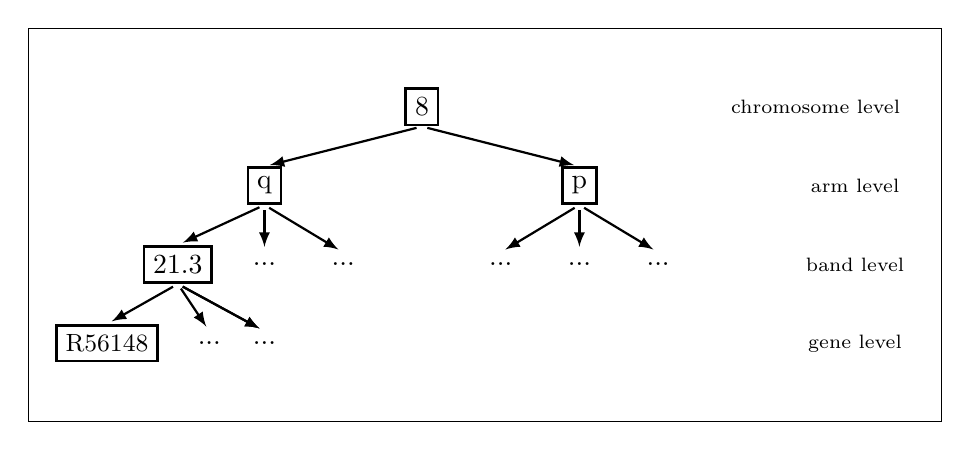
\begin{tikzpicture}
  \draw (0,-1) rectangle (11.6,4);
  \begin{scope}[draw, line width=1pt]
  \path          (5,3) node[draw] (top) {8} ;
  \path     (3,2)  node[draw] (abc) {q} ;
  \path    (7,2) node[draw] (de) {p} ;
  \path     (1.9,1) node[draw] (ab) {21.3} ;
  \path     (4,1) node[] (c) {...} ;
    \path     (3,1) node[] (h) {...} ;
  \path          (6,1) node[] (d) {...} ;
    \path          (7,1) node[] (f) {...} ;
  \path           (8,1) node[] (e) {...} ;
  \path     (1,0) node[draw] (a) {\small R56148};
    \path     (2.3,0) node[] (g) {...};
  \path            (3,0) node[] (b) {...};
    \path     (10.5,0)  node {{\scriptsize gene level}};
  \path     (10.5,1) node {{\scriptsize band level}};
  \path     (10.5,2)  node {{\scriptsize arm level}};
    \path     (10,3) node {{\scriptsize chromosome level}};
   \end{scope}
  \begin{scope}[thick, shorten >= 2pt,shorten <= 2pt, latex-]
    \draw         (abc.north) -- (top.south);
    \draw         (de.north) -- (top.south);
    \draw         (ab.north) -- (abc.south);
        \draw         (h.north) -- (abc.south);
    \draw (c.north) -- (abc.south);
    \draw (b.north) -- (ab.south);
    \draw (a.north) -- (ab.south);
    \draw (b.north) -- (ab.south);
        \draw (g.north) -- (ab.south);
    \draw (e.north) -- (de.south);
    \draw (d.north) -- (de.south);
       \draw (f.north) -- (de.south);
  \end{scope}
  \end{tikzpicture}
\end{figure}

\begin{overprint}

\onslide<1>
\begin{center}
root = general question, $\downarrow$ = more specific follow-up questions\\
\end{center}

\onslide<2>
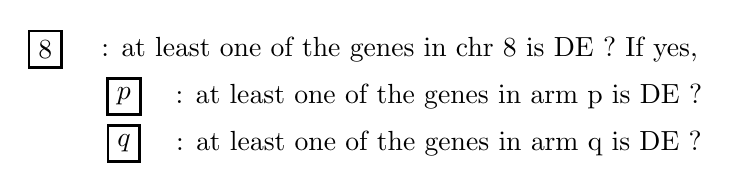
\begin{tikzpicture} \begin{scope}[draw, line width=1pt] 
\path (0,0)  node[draw] (a) {$8$};
\path (4.5,0)  node (a) {: at least one of the genes in chr 8 is DE ? If yes, };
\path (1,-.6)  node[draw] (a) {$p$};
\path (5,-.6)  node (a) {: at least one of the genes in arm p is DE ?};
\path (1,-1.2)  node[draw] (a) {$q$};
\path (5,-1.2)  node (a) {: at least one of the genes in arm q is DE ?};
 \end{scope} 
 \end{tikzpicture}
etc.

\end{overprint}

\end{frame}
% %% ==========================INHERITANCE
% \section{Inheritance procedure}
% \subsection{}
% 
% \begin{frame}
% \frametitle{Meinshausen's procedure (BMK 2008)}
% 
% \begin{overprint}
% 
%  \onslide<1>
%  
%  \bb{}{
%    start from the top: \\
%    test $ABCDE$ at level $\alpha$}\eb
%   \onslide<2>
%    \bb{}{
%    suppose $p_{ABCDE}\leq \alpha$, \\
%    test $ABC$ at $\frac{3}{5}\alpha$ and $DE$ at $\frac{2}{5} \alpha$}\eb
%    \onslide<3>
%     \bb{}{
%    suppose $p_{ABC}\leq \frac{3}{5}\alpha$ and $p_{DE}>\frac{2}{5} \alpha$}\eb
%    \onslide<4>
%     \bb{}{
%    test $AB$ at $\frac{2}{5}\alpha$ and $C$ at $\frac{1}{5}\alpha$}\eb
%    \onslide<5>
%     \bb{}{
%    suppose $p_{AB}\leq \frac{2}{5}\alpha$ and $p_{C}> \frac{1}{5}\alpha$, \\
%    test $A$ at  $\frac{1}{5}\alpha$ and $B$ at $\frac{1}{5}\alpha$}\eb
%    \onslide<6>
%     \bb{}{
%    suppose $p_{A}\leq \frac{1}{5}\alpha$ and $\frac{1}{5}\alpha < p_{B}< \frac{2}{5}\alpha$\\
%    STOP?}\eb
%   \onslide<7>
%       \bb{}{
%     \textcolor{green}{Shaffer's improvement:} if $A\cap B$ is a correct rejection, \\ at least one hypothesis is false: test $A$ and $B$ at level $\frac{2}{5}\alpha$
% }\eb
%   \onslide<8>
%       \bb{}{
%     reject A and B. \\
%     STOP!}\eb
% \end{overprint}
% 
% \begin{figure}
%   \begin{tikzpicture}
%   \draw (0,-1) rectangle (10,4);
%   \begin{scope}[draw, line width=1pt]
%     \path<1>   [blue]       (5,3) node[draw] (top) {$ABCDE$} ;
%   \path<1>[blue]    (top.east)   node {$\quad \alpha$} ;
%   \path<2>[blue] (5,3) node[draw] (top) {$ABCDE$} ;
%   \path<2->[red] (5,3) node[draw, cross out] (top) {$ABCDE$} ;
%   \path<2->[red] (5,3) node[draw] (top) {$ABCDE$} ;
%   \path<1-2>     (3,2)  node[draw] (abc) {$ABC$} ;
%   \path<2>[blue] (3,2)  node[draw] (abc) {$ABC$} ;
%   \path<2>[blue] (abc.east)  node {$\ \quad \alpha \frac{3}{5}$} ;
%   \path<3->[red] (3,2) node[draw, cross out] (abc) {$ABC$} ;
%   \path<3->[red] (3,2) node[draw] (abc) {$ABC$} ;
%   \path<1-2>     (7,2) node[draw] (de) {$DE$} ;
%   \path<2->[blue] (7,2) node[draw] (de) {$DE$} ;
%   \path<2->[blue] (de.east) node {$\ \quad \alpha \frac{2}{5}$} ;
%   \path<1-3>     (1.9,1) node[draw] (ab) {$AB$} ;
%   \path<4>[blue] (1.9,1) node[draw] (ab) {$AB$} ;
%   \path<4>[blue] (ab.east) node {$\ \quad  \alpha \frac{2}{5}$} ;
%   \path<5->[red] (1.9,1) node[draw, cross out] {$AB$} ;
%   \path<5->[red] (1.9,1) node[draw] {$AB$} ;
%   \path<1-3>     (4,1) node[draw] (c) {$C$} ;
%   \path<4->[blue] (4,1) node[draw] (c) {$C$} ;
%   \path<4->[blue] (c.east) node {$\ \quad \alpha \frac{1}{5}$} ;
%   \path          (6,1) node[draw] (d) {$D$} ;
%   \path           (8,1) node[draw] (e) {$E$} ;
%   \path     (1,0) node[draw] (a) {$A$};
%   \path<5>[blue] (1,0) node[draw] (a) {$A$};
%   \path<6>[red]  (1,0) node[draw] (a) {$A$};
%   \path<6>[red]  (1,0) node[draw, cross out] (a) {$A$};
%   \path<7>[blue] (1,0) node[draw] (a) {$A$};
%   \path<8>[red]  (1,0) node[draw] (a) {$A$};
%   \path<8>[red]  (1,0) node[draw, cross out] (a) {$A$};
%   \path<5>[blue] (a.east)node {$\ \quad \alpha \frac{1}{5}$} ;
%   \path<7>[green](a.east)node[draw] {$\ \quad \alpha \frac{2}{5}$} ;
%   \path            (3,0) node[draw] (b) {$B$};
%   \path<5->[blue]   (3,0) node[draw] (b) {$B$};
%   \path<5-6>[blue]  (b.east) node {$\ \quad \alpha \frac{1}{5}$} ;
%   \path<7>[green]    (b.east)node[draw] {$\ \quad  \alpha \frac{2}{5}$} ;
%   \path<8->[red]    (3,0) node[draw] (b) {$B$};
%   \path<8->[red]    (3,0) node[draw, cross out] (b) {$B$};
%   \end{scope}
%   \begin{scope}[thick, shorten >= 2pt,shorten <= 2pt, latex-]
%     \draw         (abc.north) -- (top.south);
%     \draw<2->[red] (abc.north) -- (top.south);
%     \draw         (de.north) -- (top.south);
%     \draw<2>[red] (de.north) -- (top.south);
%     \draw         (ab.north) -- (abc.south);
%     \draw<4->[red] (ab.north) -- (abc.south);
%     \draw (c.north) -- (abc.south);
%     \draw<4>[red] (c.north) -- (abc.south);
%     \draw (b.north) -- (ab.south);
%     \draw (a.north) -- (ab.south);
%     \draw (b.north) -- (ab.south);
%     \draw<5-6, 8>[red] (a.north) -- (ab.south);
%     \draw<5>[red] (b.north) -- (ab.south);
%         \draw<7>[green] (a.north) -- (ab.south);
%     \draw<7>[green] (b.north) -- (ab.south);
%         \draw<8>[red] (b.north) -- (ab.south);
%     \draw<4->[red] (d.north) -- (de.south);
%     \draw (e.north) -- (de.south);
%     \draw (d.north) -- (de.south);
%   \end{scope}
%   \end{tikzpicture}
% \end{figure}
% \end{frame}